%!TEX root = ../../thesis.tex
\chapter{Modellierung und Implementation}
\label{cha:modelling}

\todo[inline]{Intro}

\section{Spezifikation der Anforderungen}
\label{sec:requirements}
Der zu entwerfende Simulator soll die Ausführung ausgewählter Garbage-Collection-Algorithmen demonstrieren, sodass die einzelnen Arbeitsschritte eines Algorithmus klar erkennbar sind.
Dazu soll das in Kapitel~\ref{cha:intro} eingeführte Speichermodell realisiert werden.
Eine grafische Ausgabe visualisiert dabei den Heap als Blockgrafik: Belegte Teile des Heaps sollen von freien optisch unterschieden werden können, zudem sollen Lage und Größe der einzelnen Objekte erkennbar sein.
Die Anwenderin soll darüber hinaus die Möglichkeit haben, den Simulator zu konfigurieren:
Neben einer obligatorischen Auswahl des verwendeten Garbage-Collection-Algorithmus soll auch die Größe des Heaps sowie die Größe der erzeugten Heapobjekte einstellbar sein.
Weitere Anpassungsmöglichkeiten sind der Verzweigungsgrad der Objekte untereinander sowie die Verwaisungswahrscheinlichkeit, sodass verschiedene Objektkonstellationen betrachtet werden können.
Zuletzt soll durch eine Anpassbarkeit der Animationsgeschwindigkeit auch die Visualisierung anpassbar sein.

Aus Sicht der Softwareentwicklung ergeben sich zusätzliche Anforderungen, die für die Umsetzung der Anwendung relevant sind:
Der Simulator soll als frei verwendbare Software im Rahmen der Lehre eingesetzt werden können und beliebig anpassbar und erweiterbar sein, etwa indem Entwicklerinnen weitere Garbage-Collection-Algorithmen ergänzen.
Dies impliziert die Verwendung verschiedener Konzepte der Objektorientierung, unter anderem der Modularisierung in funktional unterscheidbare Pakete und Klassen, der Polymorphie und der generischen Programmierung.
Darüber hinaus soll die Anwendung plattformunabhängig entwickelt werden, um sie möglichst vielen Anwenderinnen zugänglich zu machen.

\section{Modellierung}
\label{sec:model}
Aufgrund der oben beschriebenen Anforderungen bietet sich die in Abbildung~\ref{fig:model} dargestellte Aufteilung in einzelne Komponenten an, auf deren Funktion im Folgenden eingegangen wird.
Bereits in Kapitel~\ref{cha:intro} wurde angemerkt, dass sich ein Programm grob in die drei Bestandteile Mutator, Allokator und Kollektor einteilen lässt.
Insofern ist es sinnvoll, diese Einteilung möglichst auch in die Modellierung einfließen zu lassen, insbesondere um verschiedene Kombinationen von Allokator und Kollektor zu ermöglichen.

\begin{figure}[h]
	\centering
	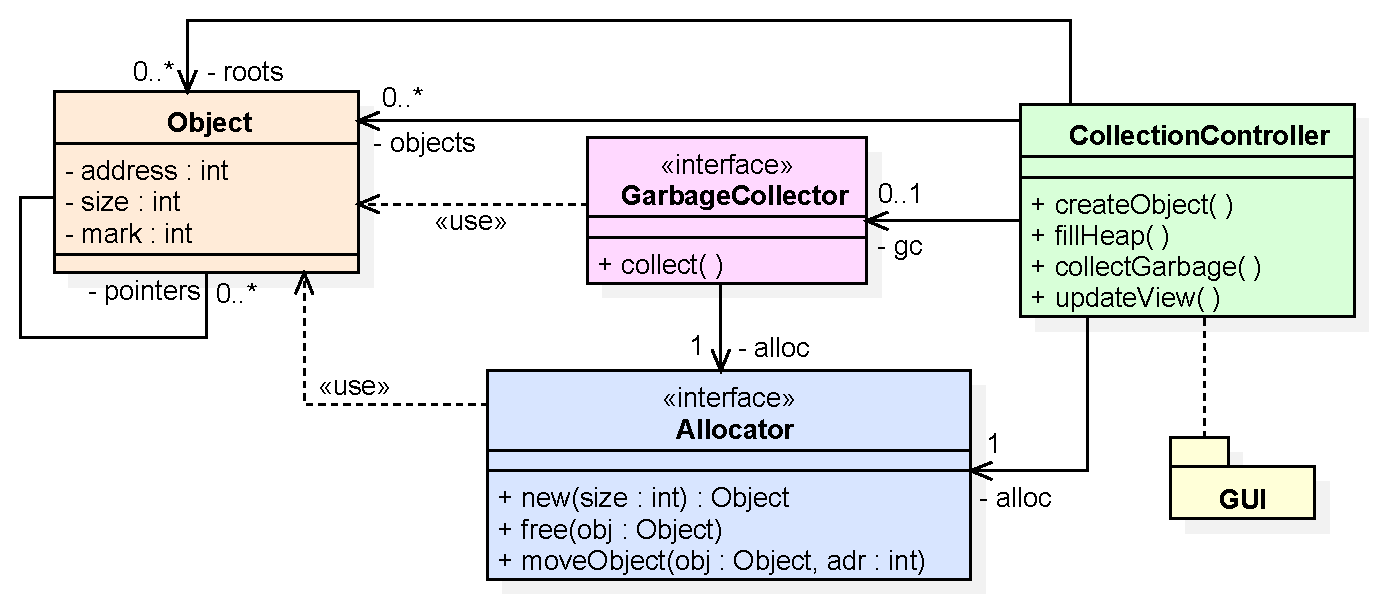
\includegraphics[scale=0.6]{img/uml/ch7-model.pdf}
	\caption[Klassendiagramm zur Modellierung von Mutator, Allokator und Kollektor]{Klassendiagramm zur Modellierung von Mutator, Allokator und Kollektor.}
	\label{fig:model}
\end{figure}

Heapobjekte werden als Instanzen einer Klasse \code{Object} modelliert und beinhalten Speicheradresse (\code{address}), Größe (\code{size}), Markierungsinformation (\code{mark}) und eine Menge \code{pointers} an Referenzen auf weitere Instanzen von \code{Object}, um die Menge \Pointers zu realisieren.
Ansonsten bieten sie keinerlei Funktionalität an.

Eine Instanz der Schnittstelle \code{Allocator} stellt die wesentlichen Dienste eines Allokators zu Verfügung.
Dazu zählt die Anforderung einer Speichermenge durch den Mutator mittels \code{new}, die Freigabe von Objekten und des durch sie belegten Speicherbereichs sowie das Verschieben eines Objekts.
Ersteres geschieht durch Übergabe der gewünschten Speichermenge und Rückgabe eines neu erzeugten Instanz von \code{Object}, die die entsprechende Speicheradresse enthält.
Der Allokator ist diejenige Instanz, die Informationen über den Füllstand des Heaps und insbesondere über die Belegung einzelner Wörter besitzt.
Die Schnittstelle \code{GarbageCollector} beschreibt die Funktionalität eines Kollektors, welche im Wesentlichen aus der Durchführung eines Garbage-Collection-Zyklus (Methode \code{collect}) besteht.
Da eine Garbage Collection die Freigabe und Verschiebung von Objekten auslösen kann, verwaltet sie genau eine Instanz von \code{Allocator}.
Die Klasse \code{CollectionController} realisiert einerseits die Aufgabe des Mutators, das heißt die Anforderung von Speicher für neue Objekte sowie die (Simulation von) Referenzmanipulationen, die zur Verwaisung von Objekten führen.
Daher besitzt sie zwei Mengen von Heapobjekten \code{objects} und \code{roots}.
\code{objects} enthält dabei sämtliche Objekte des Heaps und \code{roots}\ -- entsprechend der Menge \Roots -- alle Basisobjekte.
Zudem verwaltet sie eine \code{Allocator}-Instanz, um Speicher anfordern zu können, sowie eine \code{GarbageCollector}-Instanz zur Auslösung der Garbage Collection.
Andererseits fungiert \code{CollectionController} als Steuerklasse, um über die GUI eingehende Benutzerinteraktionen umsetzen und delegieren zu können.

Die Idee ist nun, beim Start des Simulators zunächst eine Instanz der Klasse \code{CollectionController} erzeugen.
Diese legt wiederum -- je nach ausgewählter Garbage Collection -- eine geeignete \code{Allocator}-Instanz sowie einen \code{GarbageCollector} an.
Letzterer bekommt dabei den zuvor erzeugten Allokator übergeben, sodass Kollektor und Steuerklasse auf denselben simulierten Heap zugreifen.

\section{Implementation}
\label{sec:implementation}
